On the NIF and OMEGA convergence ratios are generally inferred using x-ray imaging techniques. An example image is shown below in Figure \ref{fig:xrayImage}. 

\begin{figure}[h!]
    \centering
    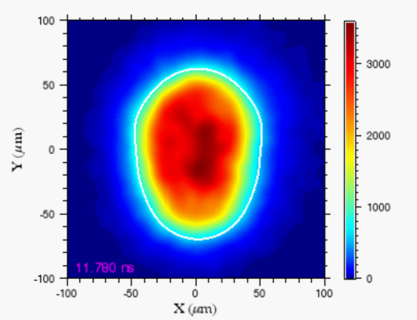
\includegraphics[scale=2.0]{Figures/xrayImage.pdf}
    \caption[Example X-ray Image]{\todo{Get a better image} X-ray self-emission image taking from the equator of NIF shot N170530. }
    \label{fig:xrayImage}
\end{figure}

From these images, a contour can be drawn at the value corresponding to 17\% of the peak intensity value. This contour shape is used to represent the size and shape of the fuel plasma. The shape can be fit to Legendre modes in the form shown in equations \ref{eq:outerR} and \ref{eq:innerR}. Obviously, in the context of a 2D image, $m$ modes have no meaning so $m$ is taken to be 0. Results are often quoted using the notation defined in equations \ref{eq:P0} and \ref{eq:Pl}.

In particular, the P0 is taken to be a representation of the fuel plasma's average radius. This is motivated by the simple fact that:
%
\begin{equation}
    \frac{1}{2\pi} \int d\theta \sum_{\ell=0}^{\infty} \Delta_\ell^0 \alpha_\ell^0 P_\ell^0(\cos\theta) = \Delta_0^0\alpha_0^0 \equiv P0
\end{equation}
%
With this radius, we can determine the convergence ratio:
%
\begin{equation}
    CR_{xray} = \frac{R_i + t_i}{P0}
\end{equation}
%
Where $R_i$ and $t_i$ are the initial inner radius and ablator thickness of the imploded capsule. 

Secondary DT neutrons can also be used to infer the convergence ratio of an implosion. Recall that regardless of asymmetries, the yield of the secondary DT neutron spectra can be used to infer the directionally averaged fuel areal density. From mass conservation we have:
%
\begin{equation}
    \int d\Omega \int dr r^2 \rho = \frac{4}{3}\pi\rho_iR_i^3
    \label{eq:massConservation}
\end{equation}
%
where $\rho_i$ and $R_i$ are the initial density and radius of the capsule. If we take the mass density radial profile to be:
%
\begin{equation}
    \rho (r) \propto \left(1-\left(\frac{r}{R}\right)^2\right)^\gamma
\end{equation}
%
It can be shown that
%
\begin{equation}
    \int dr r^2 \rho & = \frac{\Gamma(\gamma+\frac{3}{2})}{2\Gamma(\gamma+\frac{5}{2})}R^2 \int dr \rho 
\end{equation}
% 
Combining this result with equation \ref{eq:dirAveragedRhoR} and \ref{eq:massConservation} gives us:
%
\begin{equation}
    \frac{\Gamma(\gamma+\frac{3}{2})}{2\Gamma(\gamma+\frac{5}{2})}R^2 \left<\rho R\right> = \frac{1}{3}\rho_iR_i^3
\end{equation}
%
Which we can rearrange terms to show:
%
\begin{equation}
    CR_{2DTn} & = \sqrt{\frac{\left<\rho R\right>}{\rho_i R_i}} \times \sqrt{\frac{3\Gamma(\gamma+\frac{3}{2})}{2\Gamma(\gamma+\frac{5}{2})}} \times \left(1+\frac{t_i}{R_i}\right)
\end{equation}
%
As we can see, the convergence ratio is primarily proportional to the square root of the areal density ratio. There is a coefficient associated with profile effects and a coefficient needed to include the thickness of the ablator. Often times, $\gamma$ is taken to be 0 (uniform profile assumption) where the corresponding coefficient goes to 1. Other values of this coefficient are shown plotted in Figure \ref{fig:CR_Profile_Coef}.

\begin{figure}[h!]
    \centering
    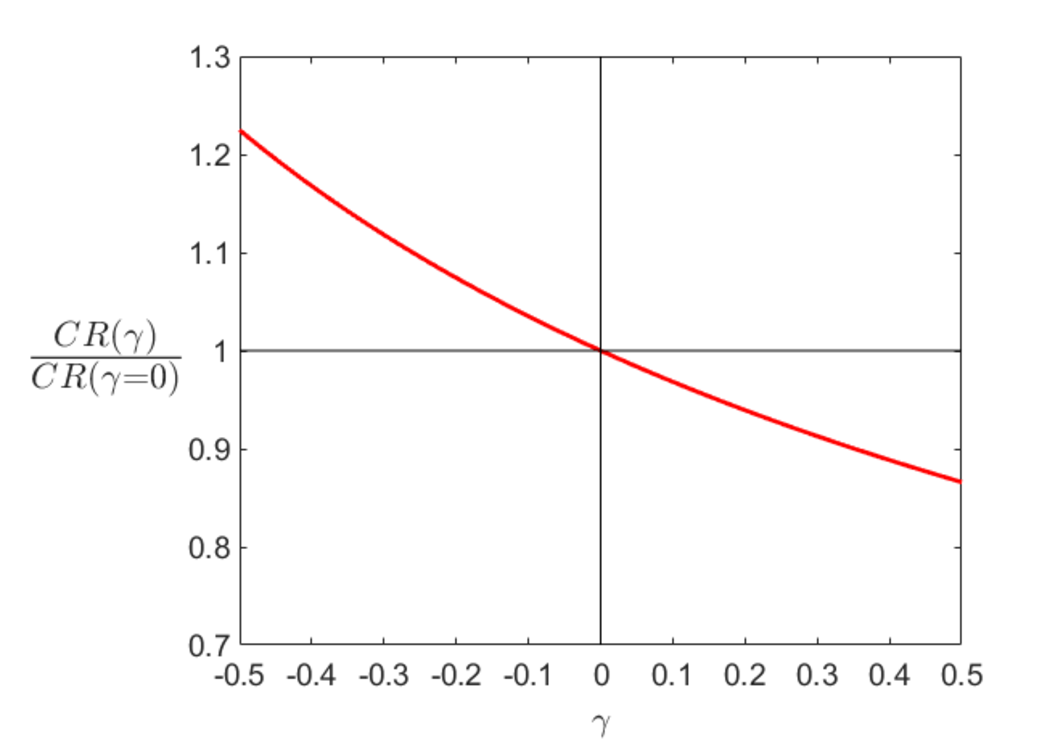
\includegraphics[scale=0.8]{Figures/CR_Profile_Coef.pdf}
    \caption[Convergence Ratio Profile Effect Coefficient]{The relative effect of profiles on the convergence ratio's correlation with the square root of the areal density ratio.}
    \label{fig:CR_Profile_Coef}
\end{figure}

As can be seen in Figure \ref{fig:CR_Profile_Coef}, the coefficient is greater than 1 for $\gamma < 0$ and less than 1 for $\gamma > 0$. What this means intuitively is that a uniform profile assumption would overestimate the true convergence ratio for profiles peaked at the center of the plasma and underestimate the true convergence ratio for profiles peaked at the edge. In this work, we will take $\gamma=0$ when inferring convergence ratios using secondary DT neutrons. 






